\leftsection{Программа 3}

\subsection{Вариант 1 (небуферизованный ввод-вывод)}
\subsubsection{Однопоточная программа}

\begin{lstlisting}[language=c, caption={Третья программа 1 (однопоточный вариант)}]
#include <stdlib.h>
#include <stdio.h>
#include <fcntl.h>
#include <unistd.h>

#include "stat.h"

#define MAX_FDS 10

struct arg
{
    int valid;
    size_t amount;
};

int main(int argc, char **argv)
{
    const struct arg arg = parse_args(argc, argv);

    if (EXIT_SUCCESS != arg.valid)
        return EXIT_FAILURE;

    int fds[MAX_FDS] = {-1};
    int rc = EXIT_SUCCESS;

    for (size_t i = 0; EXIT_SUCCESS == rc && arg.amount > i; i++)
    {
        fds[i] = open("task3.txt", O_CREAT | O_TRUNC | O_WRONLY);
        STAT_WRAP("open", print_path_stat("task3.txt"));

        if (0 > fds[i])
        {
            perror("open error\n");
            rc = EXIT_FAILURE;
        }
    }

    if (EXIT_SUCCESS == rc)
        for (char c = 'a'; 'z' >= c; c++)
        {
            write(fds[c % arg.amount], &c, sizeof(char));
            STAT_WRAP("write", print_path_stat("task3.txt"));
        }

    for (size_t i = 0; arg.amount > i; i++)
        if (0 <= fds[i])
        {
            close(fds[i]);
            STAT_WRAP("close", print_path_stat("task3.txt"));
        }

    return EXIT_SUCCESS;
}
\end{lstlisting}

\begin{figure}[h]
    \centering
    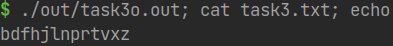
\includegraphics[width=0.7\textwidth]{task3o.png}
    \caption{Результат работы третьей программы 1.}
\end{figure}

Аналогично однопоточному варианту предыдущей программы, процесс получает
несколько независимых дескрипторов одного файла. В результате этого, при
поочередной записи символов, происходит затирание символов, расположенных
на одной позиции. Полученный файл содержит запись, формируемую с использованием
последнего файлового дескриптора.

\subsubsection{Многопоточная программа}

\begin{lstlisting}[language=c, caption={Третья программа 1 (многопоточный вариант)}]
#include <stdlib.h>
#include <stdio.h>
#include <fcntl.h>
#include <unistd.h>
#include <pthread.h>
#include <string.h>

#include "stat.h"

#define MAX_THREADS 10

struct arg
{
    int valid;
    size_t threads;
};

struct data
{
    char c;
    pthread_mutex_t mutex;
    const struct arg *arg;
};

struct handle
{
    size_t id;
    struct data *data;
};

void *thread_func(void *_arg)
{
    struct handle *arg = _arg;
    char tmp[30];
    ssize_t len;

    int fd = open("task3.txt", O_WRONLY);
    STAT_WRAP("open", print_path_stat("task3.txt"));

    if (0 > fd)
    {
        perror("open error\n");

        return NULL;
    }

    for (int run = 1, rc = EXIT_SUCCESS; EXIT_SUCCESS == rc && run;)
    {
        rc = pthread_mutex_lock(&arg->data->mutex);

        if (EXIT_SUCCESS == rc)
        {
            if ('z' < arg->data->c)
                run = 0;
            else if ((arg->data->c - 'a') % arg->data->arg->threads
                     == arg->id - 1)
            {
                len = sprintf(tmp, "thread %zu: %c\n", arg->id,
                              arg->data->c++);
                write(fd, tmp, len);
                STAT_WRAP("write", print_path_stat("task3.txt"));
            }

            if (EXIT_SUCCESS != pthread_mutex_unlock(&arg->data->mutex))
            {
                perror("mutex_unlock error\n");
                rc = EXIT_FAILURE;
            }
        }
        else
            perror("mutex_lock error\n");
    }

    close(fd);
    STAT_WRAP("close", print_path_stat("task3.txt"));

    return NULL;
}

int main(int argc, char **argv)
{
    const struct arg arg = parse_args(argc, argv);

    if (EXIT_SUCCESS != arg.valid)
        return EXIT_FAILURE;

    if (EXIT_SUCCESS != close(open("task3.txt", O_CREAT | O_TRUNC)))
        return EXIT_FAILURE;

    struct data data = {
        .c = 'a',
        .mutex = {{0}},
        .arg = &arg
    };

    if (EXIT_SUCCESS != pthread_mutex_init(&data.mutex, NULL))
    {
        perror("mutex_init error\n");
        return EXIT_FAILURE;
    }

    struct handle args[MAX_THREADS];
    pthread_t threads[MAX_THREADS];
    int rc = EXIT_SUCCESS;

    for (size_t i = 0; EXIT_SUCCESS == rc && arg.threads > i; i++)
    {
        args[i].id = i + 1;
        args[i].data = &data;

        if (EXIT_SUCCESS
            != pthread_create(threads + i, NULL, thread_func, args + i))
        {
            perror("pthread_create error\n");
            rc = EXIT_FAILURE;
        }
    }

    for (size_t i = 0; arg.threads > i; i++)
        pthread_join(threads[i], NULL);

    pthread_mutex_destroy(&data.mutex);

    return EXIT_SUCCESS;
}
\end{lstlisting}

\begin{figure}[h]
    \centering
    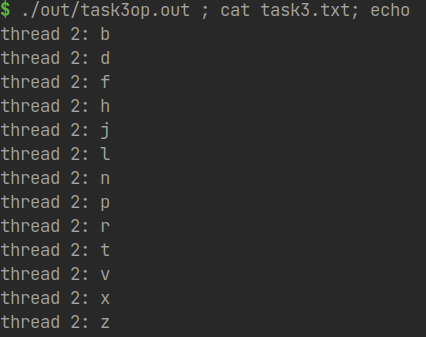
\includegraphics[width=0.7\textwidth]{task3op.png}
    \caption{Результат работы третьей программы 1.}
\end{figure}

Для обеспечения последовательной записи букв алфавита потоками в программе
используется mutex, как средство синхронизации. Это приводит к тому, что
результат выполнения одонопточной и многопоточной версий программы не
отличаются.

\subsubsection{Связь структур}

\vspace*{\fill}
\begin{figure}[h]
    \centering
    \def\svgwidth{\textwidth}
    \input{task3o.pdf_tex}
\end{figure}
\vfill

\subsection{Вариант 2 (буферизованный ввод-вывод)}
\subsubsection{Однопоточная программа}

\begin{lstlisting}[language=c, caption={Третья программа 2 (однопоточный вариант)}]
#include <stdlib.h>
#include <stdio.h>
#include <fcntl.h>
#include <unistd.h>

#include "stat.h"

#define MAX_FDS 10

struct arg
{
    int valid;
    size_t amount;
};

int main(int argc, char **argv)
{
    const struct arg arg = parse_args(argc, argv);

    if (EXIT_SUCCESS != arg.valid)
        return EXIT_FAILURE;

    FILE *fds[MAX_FDS] = {NULL};
    int rc = EXIT_SUCCESS;

    for (size_t i = 0; EXIT_SUCCESS == rc && arg.amount > i; i++)
    {
        fds[i] = fopen("task3.txt", "w");
        STAT_WRAP("fopen", print_path_stat("task3.txt"));

        if (!fds[i])
        {
            perror("fopen error\n");
            rc = EXIT_FAILURE;
        }
    }

    if (EXIT_SUCCESS == rc)
        for (char c = 'a'; 'z' >= c; c++)
        {
            fprintf(fds[c % arg.amount], "%c", c);
            STAT_WRAP("fprintf", print_path_stat("task3.txt"));
        }

    for (size_t i = 0; arg.amount > i; i++)
        if (fds[i])
        {
            fclose(fds[i]);
            STAT_WRAP("fclose", print_path_stat("task3.txt"));
        }

    return rc;
}
\end{lstlisting}

\begin{figure}[h]
    \centering
    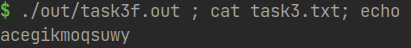
\includegraphics[width=0.7\textwidth]{task3f.png}
    \caption{Результат работы третьей программы 2.}
\end{figure}

Библиотека \verb|stdio.h| предполагает, что запись буфера на диск возможна
в одном из трех случаев:
\begin{itemize}
    \item произошло заполнение буфера;
    \item произошло закрытие файла;
    \item произошел вызов функции \verb|fflush| (принудительная запись).
\end{itemize}

Стандартный размер буфера на используемом компьютере составляет 8 КБ, из чего
следует, что запись в программе будет происходить по закрытию файла.

\begin{lstlisting}[language=c, caption={Стандартный размер буфера в библиотеке stdio}]
/* Default buffer size.  */
#define BUFSIZ 8192
\end{lstlisting}

Следовательно, содержимым файла будет результат работы с одним из библиотечных
файловых дескрипторов. \newline

\subsubsection{Многопоточная программа}

\begin{lstlisting}[language=c, caption={Вторая программа 2 (многопоточный вариант)}]
#include <stdlib.h>
#include <stdio.h>
#include <fcntl.h>
#include <unistd.h>
#include <pthread.h>
#include <string.h>

#include "stat.h"

#define MAX_THREADS 10

struct arg
{
    int valid;
    size_t threads;
};

struct data
{
    char c;
    pthread_mutex_t mutex;
    const struct arg *arg;
};

struct handle
{
    size_t id;
    struct data *data;
};

void *thread_func(void *_arg)
{
    struct handle *arg = _arg;

    FILE *fd = fopen("task3.txt", "r+");
    STAT_WRAP("fopen", print_path_stat("task3.txt"));

    if (!fd)
    {
        perror("fopen error\n");

        return NULL;
    }

    for (int run = 1, rc = EXIT_SUCCESS; EXIT_SUCCESS == rc && run;)
    {
        rc = pthread_mutex_lock(&arg->data->mutex);

        if (EXIT_SUCCESS == rc)
        {
            if ('z' < arg->data->c)
                run = 0;
            else if ((arg->data->c - 'a') % arg->data->arg->threads
                     == arg->id - 1)
            {
                fprintf(fd, "thread %zu: %c\n", arg->id, arg->data->c++);
                STAT_WRAP("fprintf", print_path_stat("task3.txt"));
            }

            if (EXIT_SUCCESS != pthread_mutex_unlock(&arg->data->mutex))
            {
                perror("mutex_unlock error\n");
                rc = EXIT_FAILURE;
            }
        }
        else
            perror("mutex_lock error\n");

    }

    fclose(fd);
    STAT_WRAP("fclose", print_path_stat("task3.txt"));

    return NULL;
}

int main(int argc, char **argv)
{
    const struct arg arg = parse_args(argc, argv);

    if (EXIT_SUCCESS != arg.valid)
        return EXIT_FAILURE;

    if (EXIT_SUCCESS != close(open("task3.txt", O_CREAT | O_TRUNC)))
        return EXIT_FAILURE;

    struct data data = {
        .c = 'a',
        .mutex = {{0}},
        .arg = &arg
    };

    if (EXIT_SUCCESS != pthread_mutex_init(&data.mutex, NULL))
    {
        perror("mutex_init error\n");
        return EXIT_FAILURE;
    }

    struct handle args[MAX_THREADS];
    pthread_t threads[MAX_THREADS];
    int rc = EXIT_SUCCESS;

    for (size_t i = 0; EXIT_SUCCESS == rc && arg.threads > i; i++)
    {
        args[i].id = i + 1;
        args[i].data = &data;

        if (EXIT_SUCCESS
            != pthread_create(threads + i, NULL, thread_func, args + i))
        {
            perror("pthread_create error\n");
            rc = EXIT_FAILURE;
        }
    }

    for (size_t i = 0; arg.threads > i; i++)
        pthread_join(threads[i], NULL);

    pthread_mutex_destroy(&data.mutex);

    return rc;
}
\end{lstlisting}

\begin{figure}[h]
    \centering
    \hspace*{\fill}
    \begin{minipage}{0.49\textwidth}
        \centering
        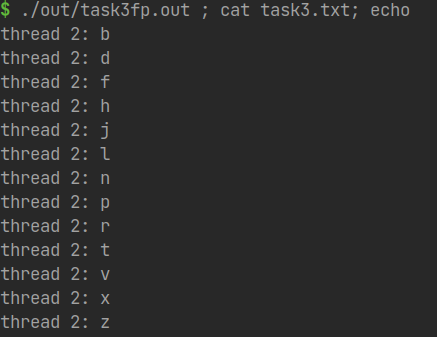
\includegraphics[width=\linewidth]{task3fp1.png}
    \end{minipage}
    \hfill
    \begin{minipage}{0.48\textwidth}
        \centering
        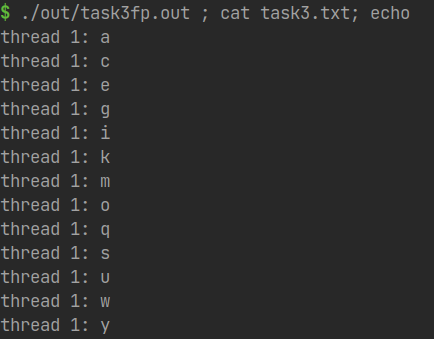
\includegraphics[width=\linewidth]{task3fp2.png}
    \end{minipage}
    \hspace*{\fill}
    \caption{Результат работы второй программы 2.}
\end{figure}

В отличие от однопоточной программы, порядок закрытия файлов в данной реализации
не определен, следовательно, в зависимости от стечения обстоятельств файл
может содержать результат работы одного из потоков.

\subsubsection{Связь структур}

\vspace*{\fill}
\begin{figure}[h]
    \centering
    \def\svgwidth{\textwidth}
    \input{task3f.pdf_tex}
\end{figure}
\vfill

\clearpage

\subsection{Вывод информации о файле с использованием stat}

\begin{figure}[h]
    \centering
    \hspace*{\fill}
    % \begin{minipage}{0.49\textwidth}
    \begin{minipage}{0.392\textwidth}
        \centering
        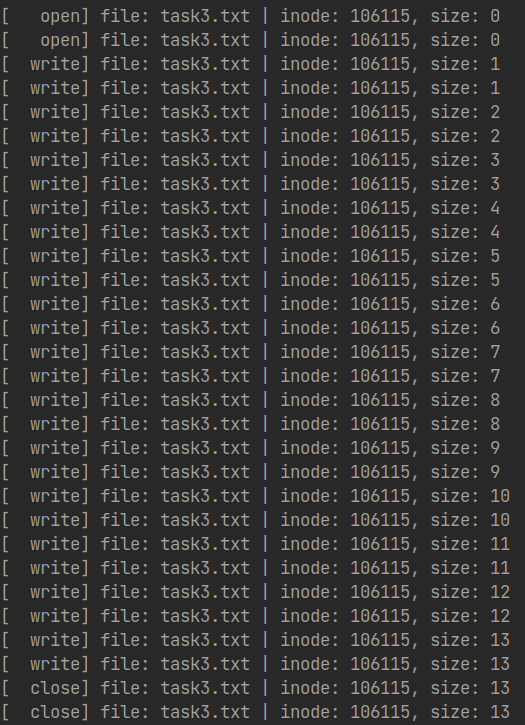
\includegraphics[width=\linewidth]{task3ostat.png}
    \end{minipage}
    \hfill
    % \begin{minipage}{0.47\textwidth}
    \begin{minipage}{0.376\textwidth}
        \centering
        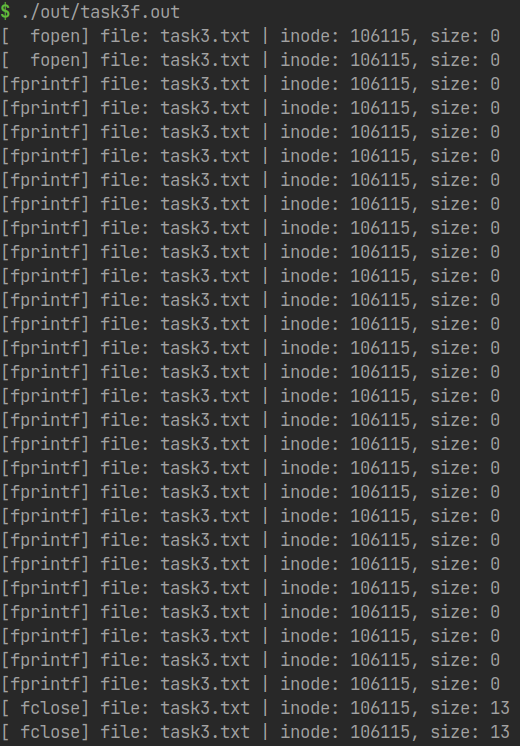
\includegraphics[width=\linewidth]{task3fstat.png}
    \end{minipage}
    \hspace*{\fill}
    \caption{Сравнение однопоточных программ.}
\end{figure}

\begin{figure}[h]
    \centering
    \hspace*{\fill}
    % \begin{minipage}{0.48\textwidth}
    \begin{minipage}{0.384\textwidth}
        \centering
        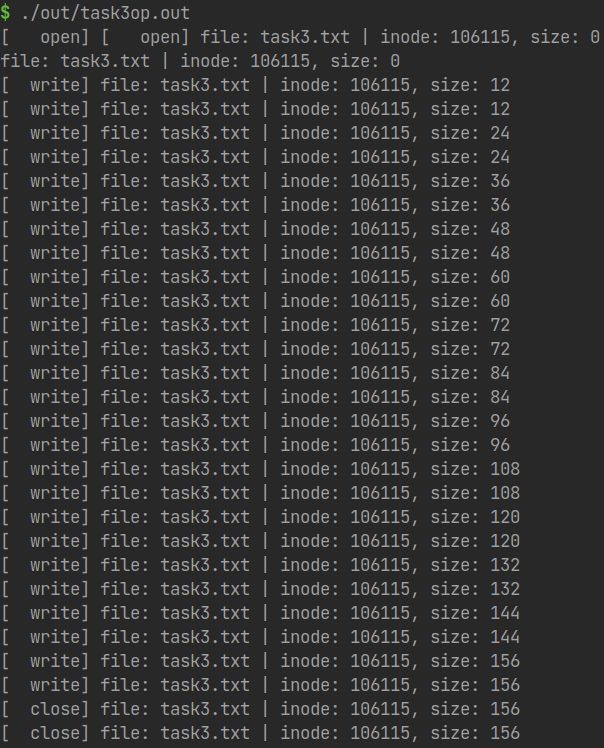
\includegraphics[width=\linewidth]{task3opstat.png}
    \end{minipage}
    \hfill
    % \begin{minipage}{0.49\textwidth}
    \begin{minipage}{0.392\textwidth}
        \centering
        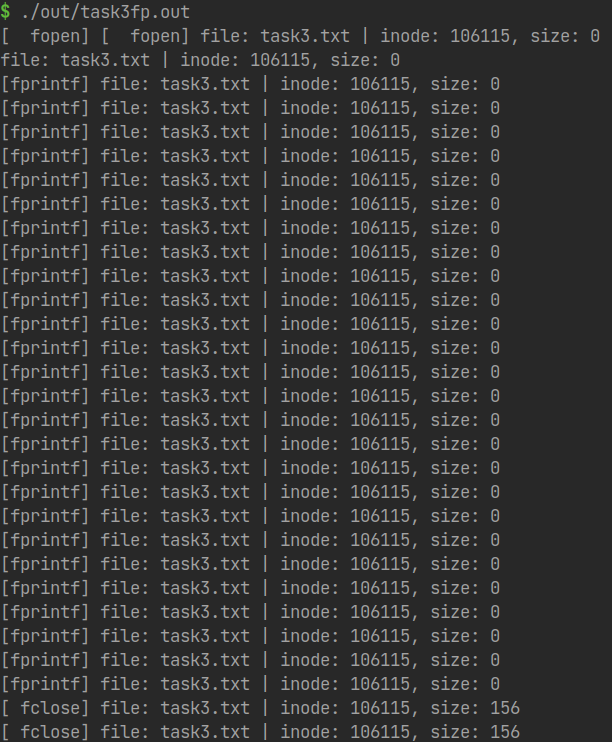
\includegraphics[width=\linewidth]{task3fpstat.png}
    \end{minipage}
    \hspace*{\fill}
    \caption{Сравнение многопоточных программ.}
\end{figure}

